\documentclass[crop,tikz]{standalone}
%
\newcommand{\Board}[4]{% x, y, w, h
  \draw[fill=brown] ({#1-(#3)/2},{#2-(#4)/2}) rectangle ++ (#3,#4);
}
%
\newcommand{\BoardOpen}[4]{% x, y, w, h
  \fill[brown] ({#1-(#3)/2},{#2-(#4)/2}) rectangle ++ (#3,#4);
  \draw ({#1-(#3)/2},{#2-(#4)/2}) -- ++ (#3,0);
  \draw ({#1-(#3)/2},{#2+(#4)/2}) -- ++ (#3,0);
}

\begin{document}
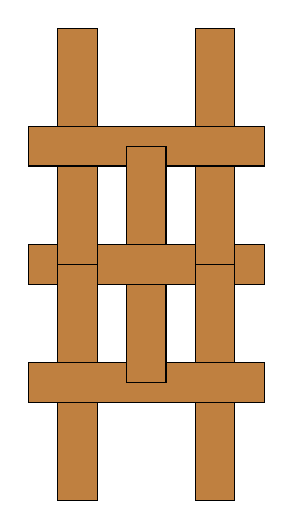
\begin{tikzpicture}
  \pgfmathsetmacro{\BoardLength}{3};
  \pgfmathsetmacro{\BoardWidth}{\BoardLength/6};
  \pgfmathsetmacro{\BoardXDistance}{(\BoardLength+\BoardWidth)/2};
  \pgfmathsetmacro{\BoardYDistance}{\BoardLength/2};
  %
  \Board{0}{-\BoardYDistance}{\BoardLength}{\BoardWidth}
  \Board{ \BoardXDistance/2}{0}{\BoardWidth}{\BoardLength}
  \Board{-\BoardXDistance/2}{0}{\BoardWidth}{\BoardLength}
  \Board{0}{0}{\BoardLength}{\BoardWidth}
  %
  \Board{ \BoardXDistance/2}{-2*\BoardYDistance}{\BoardWidth}{\BoardLength}
  \Board{-\BoardXDistance/2}{-2*\BoardYDistance}{\BoardWidth}{\BoardLength}
  \Board{0}{-2*\BoardYDistance}{\BoardLength}{\BoardWidth}
  %
  \Board{0}{-\BoardYDistance}{\BoardWidth}{\BoardLength}
  \BoardOpen{0}{-\BoardYDistance}{\BoardXDistance/2}{\BoardWidth} % correction
\end{tikzpicture}
\end{document}
